\documentclass[tikz,border=4pt]{standalone}
\usepackage{amsmath}
\usepackage{helvet}
\renewcommand{\familydefault}{\sfdefault}
\usetikzlibrary{arrows.meta,positioning,fit}
\begin{document}
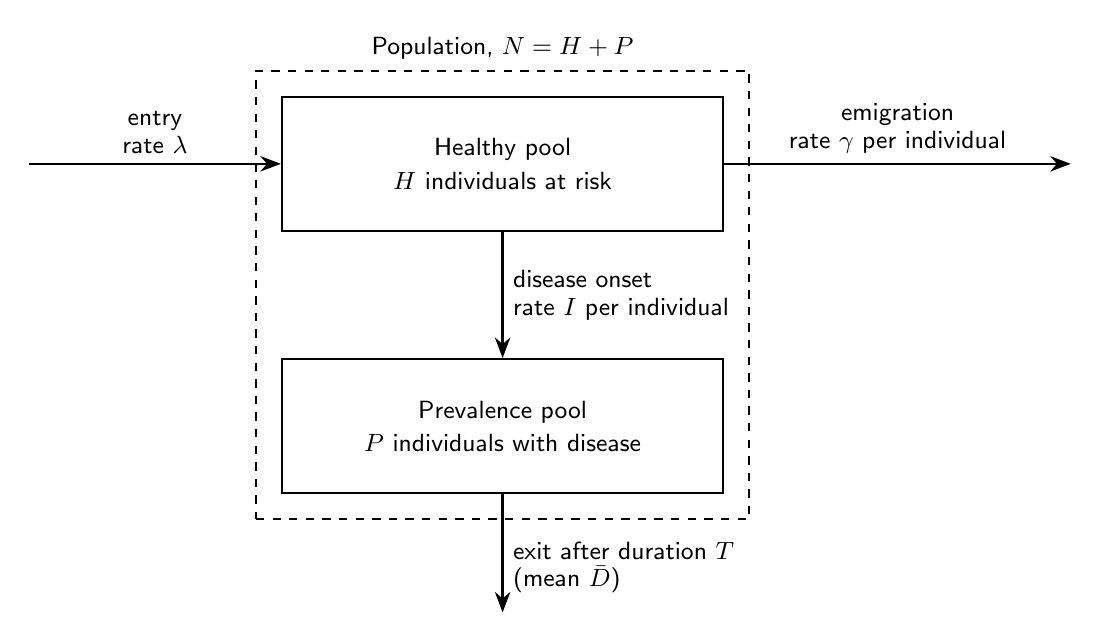
\begin{tikzpicture}[font=\small, >={Stealth[length=2.6mm]}, line width=0.9pt,
  pool/.style={draw, minimum width=5.6cm, minimum height=1.7cm, align=center}]
  \node[pool] (H) {Healthy pool\\[1pt] $H$ individuals at risk};
  \node[pool, below=1.6cm of H] (P) {Prevalence pool\\[1pt] $P$ individuals with disease};
  \node[draw, dashed, inner sep=9pt, fit=(H)(P), label={[font=\small]above:Population, $N=H+P$}] (N) {};
  \draw[->] ([xshift=-3.2cm]H.west) -- node[above, align=center]{entry\\[-1pt] rate $\lambda$} (H.west);
  \draw[->] (H.east) -- node[above, align=center]{emigration\\[-1pt] rate $\gamma$ per individual} ([xshift=4.4cm]H.east);
  \draw[->] (H.south) -- node[right, align=left]{disease onset\\[-1pt] rate $I$ per individual} (P.north);
  \draw[->] (P.south) -- node[right, align=left, pos=0.62]{exit after duration $T$\\[-1pt] (mean $\bar D$)} ([yshift=-1.5cm]P.south);
\end{tikzpicture}
\end{document}
